% Options for packages loaded elsewhere
\PassOptionsToPackage{unicode}{hyperref}
\PassOptionsToPackage{hyphens}{url}
%
\documentclass[
]{book}
\title{A Minimal Book Example}
\author{John Doe}
\date{2021-11-30}

\usepackage{amsmath,amssymb}
\usepackage{lmodern}
\usepackage{iftex}
\ifPDFTeX
  \usepackage[T1]{fontenc}
  \usepackage[utf8]{inputenc}
  \usepackage{textcomp} % provide euro and other symbols
\else % if luatex or xetex
  \usepackage{unicode-math}
  \defaultfontfeatures{Scale=MatchLowercase}
  \defaultfontfeatures[\rmfamily]{Ligatures=TeX,Scale=1}
\fi
% Use upquote if available, for straight quotes in verbatim environments
\IfFileExists{upquote.sty}{\usepackage{upquote}}{}
\IfFileExists{microtype.sty}{% use microtype if available
  \usepackage[]{microtype}
  \UseMicrotypeSet[protrusion]{basicmath} % disable protrusion for tt fonts
}{}
\makeatletter
\@ifundefined{KOMAClassName}{% if non-KOMA class
  \IfFileExists{parskip.sty}{%
    \usepackage{parskip}
  }{% else
    \setlength{\parindent}{0pt}
    \setlength{\parskip}{6pt plus 2pt minus 1pt}}
}{% if KOMA class
  \KOMAoptions{parskip=half}}
\makeatother
\usepackage{xcolor}
\IfFileExists{xurl.sty}{\usepackage{xurl}}{} % add URL line breaks if available
\IfFileExists{bookmark.sty}{\usepackage{bookmark}}{\usepackage{hyperref}}
\hypersetup{
  pdftitle={A Minimal Book Example},
  pdfauthor={John Doe},
  hidelinks,
  pdfcreator={LaTeX via pandoc}}
\urlstyle{same} % disable monospaced font for URLs
\usepackage{longtable,booktabs,array}
\usepackage{calc} % for calculating minipage widths
% Correct order of tables after \paragraph or \subparagraph
\usepackage{etoolbox}
\makeatletter
\patchcmd\longtable{\par}{\if@noskipsec\mbox{}\fi\par}{}{}
\makeatother
% Allow footnotes in longtable head/foot
\IfFileExists{footnotehyper.sty}{\usepackage{footnotehyper}}{\usepackage{footnote}}
\makesavenoteenv{longtable}
\usepackage{graphicx}
\makeatletter
\def\maxwidth{\ifdim\Gin@nat@width>\linewidth\linewidth\else\Gin@nat@width\fi}
\def\maxheight{\ifdim\Gin@nat@height>\textheight\textheight\else\Gin@nat@height\fi}
\makeatother
% Scale images if necessary, so that they will not overflow the page
% margins by default, and it is still possible to overwrite the defaults
% using explicit options in \includegraphics[width, height, ...]{}
\setkeys{Gin}{width=\maxwidth,height=\maxheight,keepaspectratio}
% Set default figure placement to htbp
\makeatletter
\def\fps@figure{htbp}
\makeatother
\setlength{\emergencystretch}{3em} % prevent overfull lines
\providecommand{\tightlist}{%
  \setlength{\itemsep}{0pt}\setlength{\parskip}{0pt}}
\setcounter{secnumdepth}{5}
\usepackage{booktabs}
\ifLuaTeX
  \usepackage{selnolig}  % disable illegal ligatures
\fi
\usepackage[]{natbib}
\bibliographystyle{plainnat}

\begin{document}
\maketitle

{
\setcounter{tocdepth}{1}
\tableofcontents
}
\hypertarget{arbeidskrav1}{%
\chapter{Arbeidskrav1}\label{arbeidskrav1}}

Placeholder

\hypertarget{introduksjon}{%
\section{Introduksjon}\label{introduksjon}}

\hypertarget{metode}{%
\section{Metode}\label{metode}}

\hypertarget{statistikk}{%
\section{Statistikk}\label{statistikk}}

\hypertarget{resultat-og-diskusjon}{%
\section{Resultat og diskusjon}\label{resultat-og-diskusjon}}

\hypertarget{vitenskapsfilosofi}{%
\chapter{Vitenskapsfilosofi}\label{vitenskapsfilosofi}}

Placeholder

\hypertarget{falsifikasjonisme}{%
\section{Falsifikasjonisme}\label{falsifikasjonisme}}

\hypertarget{hd-metoden-og-abduksjonbayesisme}{%
\section{HD-metoden og abduksjon/Bayesisme}\label{hd-metoden-og-abduksjonbayesisme}}

\hypertarget{replikasjonskrisen}{%
\section{Replikasjonskrisen}\label{replikasjonskrisen}}

\hypertarget{study-design}{%
\chapter{Study-Design}\label{study-design}}

Placeholder

\hypertarget{inntroduksjon}{%
\section{Inntroduksjon}\label{inntroduksjon}}

\hypertarget{metode-1}{%
\section{Metode}\label{metode-1}}

\hypertarget{analyzing-repeated-measures-experiments}{%
\chapter{Analyzing repeated measures experiments}\label{analyzing-repeated-measures-experiments}}

\hypertarget{inntroduksjon-1}{%
\section{Inntroduksjon}\label{inntroduksjon-1}}

I denne oppgaven skal jeg analysere, diskutere og forske på artikler som undersøker effekten av styrketrening på muskelstyrke og muskelvekst.~~\\
Forskning på styrketrening har vist det det forbedrer muskelstyrke, muskel masse, beintetthet og bindevevstykkelse \citep{kraemer2002a}. For å designe et treningsprogram for styrketrening krever det at man tar en del variabler til betraktning, dette inkluderer, treningsfrekvens, intensitet og volum av programmet \citep{hass2001a}. Innenfor forskningen på styrketrening er det stor forskjell hva er fokuset, og noe av det mest interessante er å se på forskjellen mellom antall sett, som har blitt gjort i flere studier \citep{krieger2010a}. Tidligere har det blitt argumentert for at ett sett (single- sett) per øvelse er alt som er nødvendig for hele populasjonen og at man ikke får større utbytte av flere sett \citep{carpinelli1998c}. Mens flere ander studier har argumentert for at det er et større utbytte av flere sett (multiple- sett) per øvelse \citet{galvão2005a}; \citet{humburg2007e}. Ettersom det er motstridende artikler innenfor dette området ønsker jeg i denne studien å undersøke om det er en større effekt i å trene multiple- sett mot single- sett når det kommer til utvikling av muskelstyrke og muskelvekst.

\hypertarget{metode-2}{%
\section{Metode}\label{metode-2}}

\hypertarget{forsuxf8kspersoner}{%
\subsection{Forsøkspersoner}\label{forsuxf8kspersoner}}

I denne studien var det med 41 deltakere mellom 18 og 40, både kvinner og menn. Kvalifikasjonskriteriet var å ikke røyke, og andre ekstra kriterier var intoleranse til lokal bedøvelse, en treningshistorikk på mer enn en ukentlig styrketreningsøkt i løpet av de siste 12 måneder, nedsatt muskelstyrke på grunn av nåværende eller tidligere skade, og inntak av medisiner som kunne påvirke styrketreningen. 7 deltakere ble utelukket fra studien ettersom de ikke oppfylte kravet om å fullføre minst 85\% av de planlagte treningsøktene. På Baseline var det ingen signifikant forskjell mellom gruppene som kunne føre til fordeler/ ulemper i testen. Beinøvelser ble utført på ett og ett bein for å kunne tillate for individuelle forskjell i treningsvolum. For hver deltaker ble det randomisert tildelt styrkeøvelser av enten ett sett (single- sett) eller tre sett (multiple- sett) for hvert bein. Muskelstyrken ble målt ved baseline og etter treningsintervensjonen. Muskelbiosien ble målt fra begge bein (vastus lateralis) ved baseline og etter 12 uker med trening i uthvilt tilsand.

\hypertarget{treningsprotokol}{%
\subsection{Treningsprotokol}\label{treningsprotokol}}

Før alle treningsøktene ble det utført en standardisert oppvarmingsrutine som inneholdt 5 min sykling og 10 repetisjoner med kroppsvekt av pushups, situps, rygghev og squats og 10 repetisjoner på 50\% av 1RM på hver øvelse de skal trene. Beinøvelsene ble utført i følgende rekkefølge: ettbeinsbeinpress, kne fleksjon og kneekstensjon utført som enten single- sett eller multiple- sett. Etter beinøvelsene utførte deltakerne to sett av bilatteral benkpress, nedtrekk og enten skulderpress eller sittende roing. Pausene mellom settene var på 90- 180 sekunder. Intensiteten på treningsøktene ble gradvis økt gjennom treningsperioden, deltakerne utførte 10RM de første 2 ukene, etterfulgt av 8RM i 3 uker og 7 uker med 7RM. Treningsøktene med maksimal innsats hadde minst 48t mellom og treningsøkter og submaksimale økter hadde 24t mellom. For å hjelpe med restitusjonen ble en standardisert drikke gitt etter hver øvelse.

Maksimal styrke ble beskrevet som 1RM i ettbeinsbeinpress og kneekstensjon. Testen for hver øvelse startet med en standardisert spesifikk oppvarming før 1RM ble funnet ved å øke motstanden progressivt til deltakeren ikke lenger klarte å løfte vekten.

Tverrsnittarealet til musklene i quadriceps (vastus lateralis, medialis, intermedius og rectus femoris) ble testet før og etter treningsperioden med MRI- scan. Kroppssammensetning ble bestemt før og etter treningsperioden ved bruk av en DXA- scan. Før MRI og DXA målingene måtte deltakerne være fastende i 2timer og måtte unngå hard fysisk aktivitet 48t før. ~

\hypertarget{statestikk}{%
\subsection{Statestikk}\label{statestikk}}

All deskriptiv data er presentert som et gjennomsnitt av prosentvis ending med standardavvik ved mindre annet er oppgitt. p- verdier er regnet ut ved en ANCOVA modell, på endringsscoren fra post til pre. Statistiske tester ble utført i RStudio (versjon RStudio 1.4.1717; R Foundation for Statistics Computing, Vienna, AT)

\hypertarget{resultater}{%
\section{Resultater}\label{resultater}}

Totalt, førte 12 uker med styrketrening til en signifikant økning i muskelstyrke på 31±14\% for multiple- sett og en økning på 25±13\% for multiple- sett (P\textless0,001). Økningen i muskelvekst var også signifikant på 3,3±4\% for multiple- sett og 2±4\% for single- sett (P\textless0,001).

\begin{figure}
\centering
\includegraphics{_main_files/figure-latex/Prosentvis økning figur dexa-1.pdf}
\caption{(\#fig:Prosentvis økning figur dexa)Figur 1 viser prosentvis økning ved multiple- sett og singe- sett}
\end{figure}

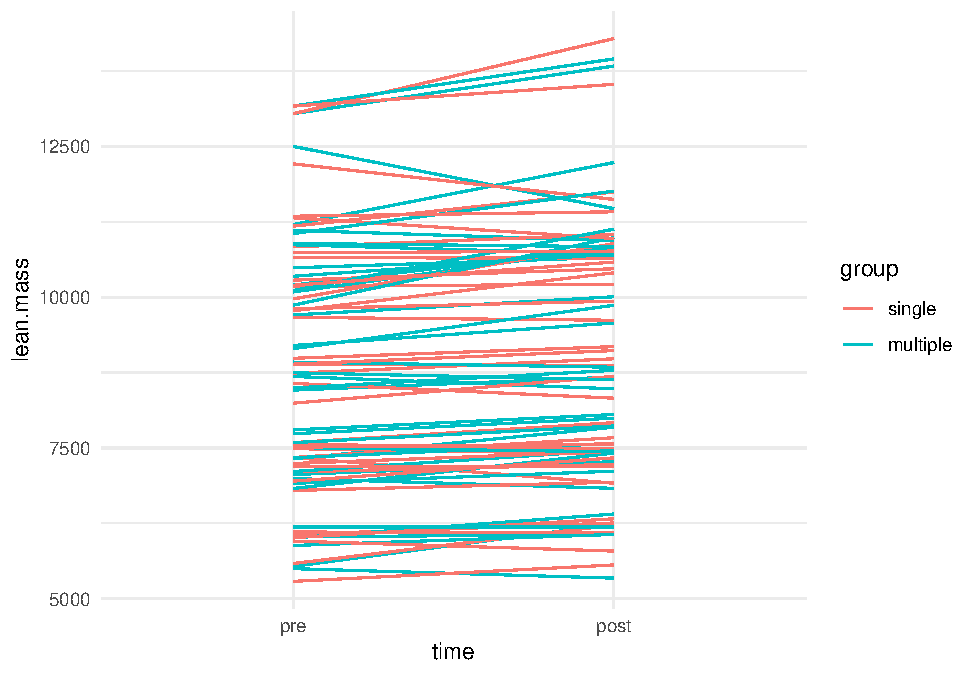
\includegraphics{_main_files/figure-latex/unnamed-chunk-4-1.pdf}

\includegraphics{_main_files/figure-latex/Prosentvis økning figur styrke-1.pdf}

\hypertarget{diskusjon}{%
\section{Diskusjon}\label{diskusjon}}

I denne studien viste det at multiple- sett styrketrening førte til bedre økning i muskelstyrke og muskelvekst enn single- sett trening. Dette resultatet stemmer overns med andre studier som har funnet at flere sett er bedre enn en \citep{galvão2005e, humburg2007c}.

Likevel samsvarer ikke resultatet i denne studien med \citep{carpinelli1998d}. Der kom de frem til at det ikke var noen signifikant forskjell i størrelsen på styrke økningen mellom 1- sett og multiple sett. I studien til \citep{carpinelli1998b} så de på studien til \citep{reid1987a} som fant ut at den gjennomsnittlige økningen i styrke var på 17,7\% for single- sett gruppen og på 17,9\% multiple- sett. Sammenlignet med vårt resultat som var på henholdsvis 25\% og 31\% på single- sett og multiple- sett. Disse forskjellene i konklusjon kan muligens bli forklart av \citep{galvão2005d} konkluderer med at styrketrening med single- sett øvelser er nok til å signifikant øke muskel funksjon, selv om muskelstyrke vil bli bedre ved et høyere treningsvolum som multiple- sett gir.

\hypertarget{konklusjon}{%
\subsection{Konklusjon}\label{konklusjon}}

Totalt sett viste denne studien at multiple- sett ga en bedre økning i muskelstyrke og muskelvekst sammenlignet med single- sett. Selv om begge gruppene hadde økning vil det kunne være mer hensiktsmessig å trene styrketrening med multiple- sett.

\hypertarget{footnotes-and-citations}{%
\chapter{Footnotes and citations}\label{footnotes-and-citations}}

\hypertarget{footnotes}{%
\section{Footnotes}\label{footnotes}}

Footnotes are put inside the square brackets after a caret \texttt{\^{}{[}{]}}. Like this one \footnote{This is a footnote.}.

\hypertarget{citations}{%
\section{Citations}\label{citations}}

Reference items in your bibliography file(s) using \texttt{@key}.

For example, we are using the \textbf{bookdown} package \citep{R-bookdown} (check out the last code chunk in index.Rmd to see how this citation key was added) in this sample book, which was built on top of R Markdown and \textbf{knitr} \citep{xie2015} (this citation was added manually in an external file book.bib).
Note that the \texttt{.bib} files need to be listed in the index.Rmd with the YAML \texttt{bibliography} key.

The RStudio Visual Markdown Editor can also make it easier to insert citations: \url{https://rstudio.github.io/visual-markdown-editing/\#/citations}

\hypertarget{blocks}{%
\chapter{Blocks}\label{blocks}}

Placeholder

\hypertarget{equations}{%
\section{Equations}\label{equations}}

\hypertarget{theorems-and-proofs}{%
\section{Theorems and proofs}\label{theorems-and-proofs}}

\hypertarget{callout-blocks}{%
\section{Callout blocks}\label{callout-blocks}}

\hypertarget{sharing-your-book}{%
\chapter{Sharing your book}\label{sharing-your-book}}

Placeholder

\hypertarget{publishing}{%
\section{Publishing}\label{publishing}}

\hypertarget{pages}{%
\section{404 pages}\label{pages}}

\hypertarget{metadata-for-sharing}{%
\section{Metadata for sharing}\label{metadata-for-sharing}}

  \bibliography{book.bib,packages.bib}

\end{document}
